% !TeX root = ../main.tex

\section{Additional Tools}

\subsection{Lag Plot}

One tool that Lawler et al use for data interpretation and model selection is a lag plot. A lag plot is a special case of a scatter plot where the $x$ coordinate of each point corresponds to a datum in a time series (except for the last one), and the $y$ coordinate corresponds to the datum directly after it. In the case of the CarHMM, $(d_t,d_{t+1})$ is plotted for every $t \in \{1, \ldots T-2\}$. If there is no auto-correlation within a given behavioral state, the lag plot should look like a group of spherically symmetric droplet patterns along the line $y=x$, and the number of droplets should correspond to the number of behavioral states. However, if there is significant auto-correlation within states, the droplets will be ``smeared" along the $y=x$ line and the number of behavioral states will be less clear. The lag plot is a good diagnostic tool to visually determine the number of behavioral states in an HMM and whether it is necessary to model within-state autocorrelation using the CarHMM. A lag plot for the killer whale case study is shown in figure (\ref{fig:lag}).

\subsection{Data Interpolation}

As mentioned earlier, the use of an HMM or CarHMM requires observations that are equispaced in time. However, this requirement in not always satisfied for real-world data, especially in the case of marine mammals, where the location of an animal is often only known when that animal comes to the surface. Lawler et al suggest linear interpolation as a solution to this issue, but warn that the uniform time step used for interpolation must be chosen with care. If the time step is too long, then the data will be over-smoothed and important information will be lost from the animal's dynamics. The number of effective observations will also be significantly less than the original data set. If the uniform time step is too short, however, then many interpolated observations will occur on the same line segment, resulting in repetitive step lengths and turning angles equal to zero. See figure (\ref{fig:interpolation}) for a visualization of both issues. To deal with this, Lawler et al. suggest using the following procedure:

\begin{enumerate}
	\item Pick a uniform time step $\Delta t_u$ and interpolate the path of the animal accordingly. Lawler et al suggest that $\Delta t_u$ be somewhere between the median and $3^{rd}$ quartile of all time steps in the raw data set. 
	\item Pick a ``group cutoff level" $\Delta t_g$. Divide observations into groups that are separated by time steps larger than $\Delta t_g$, and treat each group as an independent time series. Lawler et al suggest that $\Delta t_g$ be larger than $\Delta t_u$ to prevent fragmenting the observations too much, but less than $2*\Delta t_u$ to avoid having many interpolated points lie on the same line segment between true observations. Figure (\ref{fig:interpolation_group}) visualizes the issues of selecting $\Delta t_g$ to be too small or too large.
\end{enumerate} 

\begin{figure}[h!]
	\centering
	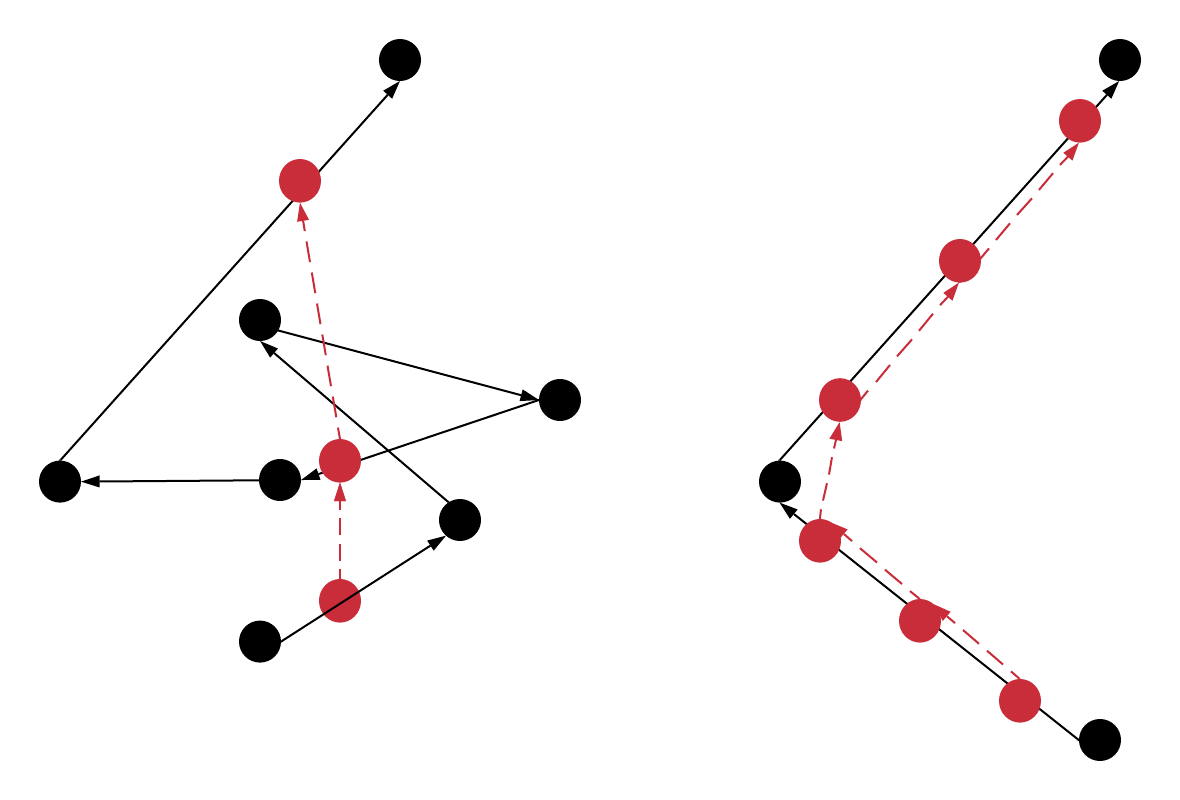
\includegraphics[height=3in]{../Plots/Interpolation.png}
	\caption{Consequences of picking $\Delta t_u$ too large (left) or too small (right). The observed track is shown in black and the interpolated track is shown in red. If $\Delta t_u$ is too large, then the true path will be over-smoothed and information about the animal's path will be lost. If $\Delta t_u$ is too small, then multiple interpolated points will appear on the same line segment, resulting in repeated step sizes and zero turning angles.}
	\label{fig:interpolation}
\end{figure}

\begin{figure}[h!]
	\centering
	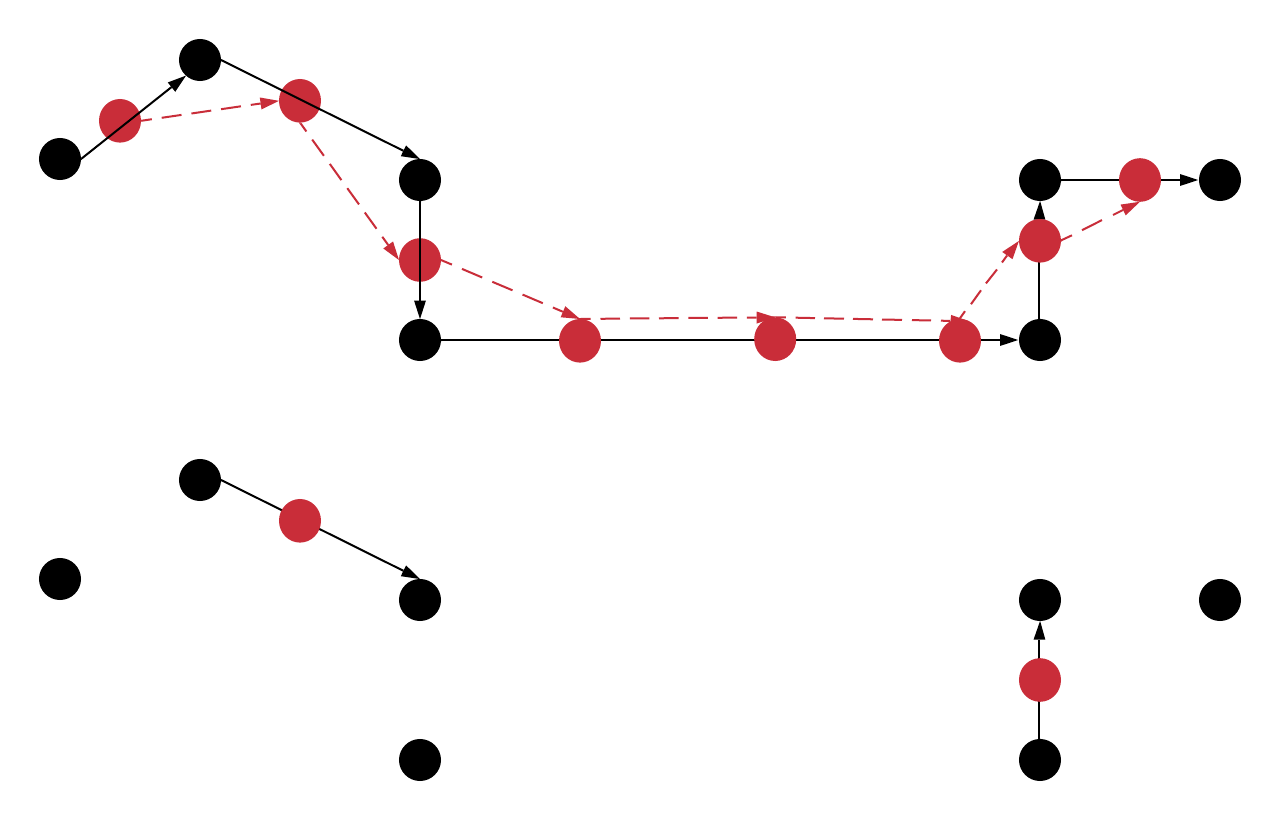
\includegraphics[height=3in]{../Plots/Interpolation_Group.png}
	\caption{Consequences of picking $\Delta t_g$ too large (above) or too small (below). The observed track is shown in black and the interpolated track is shown in red. If $\Delta t_g$ is too large, then many interpolated points will appear on some line segments, resulting in repeated step lengths and turning angles of zero degrees. If $\Delta t_g$ is too small, then many groups will appear and interpolated points not be able to create paths with turning angles.}
	\label{fig:interpolation_group}
\end{figure}

Even with the above restrictions, there is a considerable amount of freedom in choosing $\Delta t_u$ and $\Delta t_g$. Therefore, Lawler et al. introduce the two statistics to measure the quality of the choice of $\Delta t_u$ and $\Delta t_g$:

$$n_{prop} = \frac{\text{\# of interpolated points}}{\text{\# of observed locations}}$$

$$n_{adj} = \frac{\text{\# of interpolated points} - 2 \cdot \text{\# of groups}}{\text{\# of observed locations} - 2}$$

$n_{prop}$ measures the ratio of interpolated points to observed data points, while $n_{adj}$ measures the ratio of interpolated points that appear in the likelihood calculation to the number of observations that \textit{would} appear in the likelihood calculation had the data not been interpolated. Twice the number of groups is subtracted from the numerator and denominator of $n_{adj}$ because the first and last points of a group have no turning angle associated with them. Lawler et al claim that $n_{prop}$ and $n_{adj}$ should both be as close to one as possible. If these values are much larger than one, the uniform step size may be too small, resulting in replicated (or at least highly correlated) step lengths and turning angles close to zero. If these statistics are much less than one, the uniform step size may be too large, resulting in over-smoothing of the data and lost information.

Lawler et al comment that auto-correlation within the step length sequence is induced by interpolation but claim that further investigation is needed to discover the cause. To establish intuition behind this auto-correlation, suppose an interpolated point $\bfY'_s$ is equal to $\psi_s \bfY_t + (1-\psi_s) \bfY_{t+1}$, another interpolated point $\bfY'_{s+1}$ is equal to $\psi_{s+1} \bfY_{t+1} + (1-\psi_{s+1}) \bfY_{t+2}$, and a third interpolated point $\bfY'_{s+2}$ is equal to $\psi_{s+2} \bfY_{t+2} + (1-\psi_{s+2}) \bfY_{t+3}$, where $0 \leq \psi_s,\psi_{s+1},\psi_{s+2} \leq 1$. This must be the case since a linearly interpolated point is simply a convex combination of two observations. Then, we have:
%
\begin{align*}
	d'_s &= ||\bfY'_{s+1} - \bfY'_s|| \\
	%
	&= ||\psi_{s+1} \bfY_{t+1} + (1-\psi_{s+1}) \bfY_{t+2} - \psi_s \bfY_t - (1-\psi_s) \bfY_{t+1} || \\
	&= ||\psi_{s+1}(\bfY_{t+1} - \bfY_{t+2}) + \psi_s(\bfY_{t+1} - \bfY_t) + \bfY_{t+2} - \bfY_{t+1} ||  \\
	%
	&= ||(1-\psi_{s+1})(\bfY_{t+2} - \bfY_{t+1}) + \psi_s(\bfY_{t+1} - \bfY_t)||
\end{align*}
%
Similarly:
%
$$d'_{s+1} = ||(1-\psi_{s+2})(\bfY_{t+3} - \bfY_{t+2}) + \psi_{s+1}(\bfY_{t+2} - \bfY_{t+1})||$$
%
Both $(1-\psi_{s+1})$ and $\psi_{s+1}$ are positive, and the term $\bfY_{t+2} - \bfY_{t+1}$ shows up in both $d'_s$ and $d'_{s+1}$, so intuitively $d'_s$ and $d'_{s+1}$ should co-vary with one another in most cases. This provides evidence that, in general, the sequence of interpolated step-lengths $\bfD'$ exhibits more auto-correlation than the observed step lengths $\bfD$. It is therefore useful to model auto-correlation using the CarHMM if a uniform time grid is used to interpolate observations.


\subsection{Step-Size Normalization}

Lawler et al recommend dividing all step lengths by the mean observed step length to eliminate units and allow for easy comparison across data sources and animals. This process should be done with care, however, since scaling a random variable can sometimes change its distribution. Luckily, step length in the CarHMM is modeled using a gamma distribution, and gamma random variables still follow a gamma distribution when scaled by a constant. Step-size standardization can only be done if the analysis is done offline, since the mean step length is in flux for online analysis.  